\documentclass[a4paper,11pt,fleqn]{article}%fleqn pour aligner les equations à gauche
\usepackage{graphicx}
\usepackage[utf8]{inputenc}  
\usepackage[T1]{fontenc}
\usepackage{lscape}

\usepackage{tgheros,textcomp}%Police Arial
\renewcommand{\familydefault}{\sfdefault}

%\setlength{\mathindent}{0pt}%indentation dans math = 0

\usepackage[top = 1cm, bottom = 2cm, left = 1cm, right = 1cm]{geometry}
\usepackage{titlesec}
%\setcounter{secnumdepth}{4}
\usepackage{xcolor}
\usepackage{amssymb} %double flèche de réaction
\usepackage{mathrsfs}%farraday
\usepackage{xtab}%tableau sur plusieurs pages
\usepackage{esvect}%grands vecteurs

\usepackage[version=4]{mhchem} %equations chimiques

\usepackage{array}
\usepackage{chemfig}
\usepackage{multirow}
%\usepackage{sectsty}

\usepackage{caption}
\usepackage{adjustbox}
\usepackage[labelformat=simple]{subfig}
\usepackage{float}


\usepackage{amsmath}
\usepackage{amssymb}
\usepackage[cal=boondoxo]{mathalfa} 
\usepackage{enumitem}
\usepackage{lastpage}
\usepackage{tcolorbox}
\usepackage{siunitx}
\usepackage[european, straightvoltages, RPvoltages]{circuitikz}
\usepackage{tikz}
\usetikzlibrary{shapes.geometric}
\usetikzlibrary{calc}
\usetikzlibrary{automata,positioning}
\usepackage{multicol}
\usepackage{eqnarray}
\usepackage{tabularx,colortbl}%colorer fond cellules

\sisetup{
	detect-all,
	output-decimal-marker={,},
	group-minimum-digits = 3,
	group-separator={~},
	number-unit-separator={~},
	inter-unit-product={~}
} %setup pour SIunitx

\usepackage{listings}%pour insérer le code python
\definecolor{codegreen}{rgb}{0,0.6,0}
\definecolor{codegray}{rgb}{0.5,0.5,0.5}
\definecolor{codepurple}{rgb}{0.58,0,0.82}
\definecolor{backcolour}{rgb}{0.95,0.95,0.92}


\titleformat{\section}
{
\vspace{.8ex}%
\normalfont \bfseries \large}
{\thesection.}{.5em}{\bfseries}

\renewcommand{\thesection}{\arabic{section}}
\titlespacing{\section}{0pt}{1em}{.5em}
\renewcommand{\thesubsection}{\hspace{1cm}\alph{subsection}.}
\renewcommand\thesubfigure{\textbf{Document \arabic{subfigure} :}}

\title{\vspace{-1cm}\large 
	\begin{tabular}{|>{\centering}m{5cm}|>{\centering}m{8cm}|>{\centering\arraybackslash}m{4cm}|}
		\hline
		Activité Expérimentale 1 & \textbf{\textsc{Synthèse}} &  Chapitre 9 \\
		\hline
\end{tabular}}
\date{}

\newpagestyle{mystyle}{%
	\setfoot{ROSALIE}{\thepage\,$|$\,\pageref{LastPage}}{}
}
\renewpagestyle{plain}{%
	\setfoot{ROSALIE}{\thepage\,$|$\,\pageref{LastPage}}{}
}

\pagestyle{mystyle}

\newenvironment{itemize*}%
{\begin{itemize}[label=$-$,labelindent=0pt, leftmargin=*,topsep=0pt]%
		\setlength{\itemsep}{0pt}%
		\setlength{\parskip}{0pt}}%
	{\end{itemize}}

\newenvironment{itemize**}%
{\begin{itemize}[label=,labelindent=0pt, leftmargin=*,topsep=0pt]%
		\setlength{\itemsep}{0pt}%
		\setlength{\parskip}{0pt}}%
	{\end{itemize}}

\renewcommand{\arraystretch}{1.5}

\begin{document}
	\maketitle
	\vspace{-2.2cm}
	\fbox{\begin{minipage}{.45\linewidth}
		\textbf{Document 1 : Le chauffage à reflux}\\
		Ce dispositif permet le chauffage du milieu réactionnel sans perte de matière.\\
		\begin{center}
			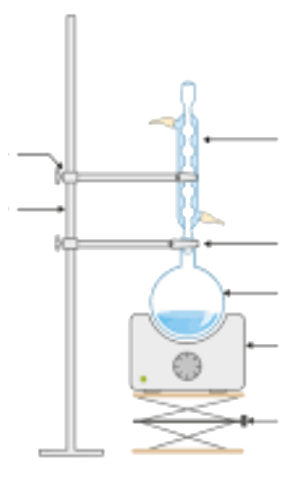
\includegraphics[scale =.5]{Ressources/TSPE_C13_AE1_Fig1.png}
		\end{center}
	\end{minipage}}
	\fbox{\begin{minipage}{.45\linewidth}
		L'essentiel du protocole est présenté dans le manuel Nathan p. 204.\\
		\vspace{1cm}
		
		\textbf{Le réfrigérant :}\\
		Le chauffage réalisé entraîne la formation de vapeurs. Le réfrigérant va condenser ces vapeurs et les faire tomber dans le mélange. Il n'y a donc pas de perte de matière et on limite grandement la sortie d'espèces chimiques volatiles et parfois dangereuses.\\
		\vspace{1cm}
		
		\textbf{Système élévateur :}\\
		Il permet l'arrêt du chauffage lorsque l'on baisse le chauffe-ballon. On peut ainsi réagir de manière plus sécurisée en cas de surchauffe.
        \vspace{1.9cm}
	\end{minipage}}

\vspace{1cm}
\noindent \begin{minipage}{\linewidth}
	
	\textbf{Document 2 : Composition des mélanges réactionnels et résultats obtenus}\\
	\emph{Remarque : le volume titré tient compte de l'ajout de \SI{200}{mL} d'eau distillée glacée.}\\
	\renewcommand{\arraystretch}{1.5}
	\centering
	\begin{tabular}{|>{\centering}m{7cm}|>{\centering}m{3cm}|>{\centering}m{3cm}|>{\centering\arraybackslash}m{3cm}|}
		\hline
		\textbf{Mélange} & \textbf{1} & \textbf{2} & \textbf{3}\\
		\hline 
		Volume d'alcool benzylique (\unit{\milli\liter}) & 10,0 & 10,0 & 10,0\\
		\hline
		$n(alcool)_i$ (\unit{\milli\mol}) & & &\\
		\hline
		Volume d'acide éthanoïque (\unit{\milli\liter}) & 5,5 & 11,0 & 55,0\\
		\hline
		$n(AH)_i$ (\unit{\milli\mol}) & & &\\
		\hline
		Volume titré (\unit{\milli\liter}) & 20,0 & 10,0 & 1,0\\
		\hline
		Volume de soude versé à l'équivalence $V_E$ (\unit{\milli\liter})& & &\\
		\hline
		$n(AH)_{\text{titré}}$ (\unit{\milli\mol}) & & &\\
		\hline 
		Coefficient multiplicateur & 10,8 & &\\
		\hline
		$n(AH))_f$(\unit{\milli\mol}) & & &\\
		\hline
		$n(ester)_f$ (\unit{\milli\mol}) & & &\\
		$n(ester)_{max}$ (\unit{\milli\mol}) & & &\\
		\hline Rendement $\eta$ (\%) & & &\\
		\hline
	\end{tabular}
\end{minipage}

\noindent \begin{minipage}{\linewidth}
	\textbf{Document 3 : Tableau d'avancement de la réaction}\\
	\renewcommand{\arraystretch}{1.5}
	\begin{tabular}{|>{\centering}m{4cm}|>{\centering}m{3cm}|>{\centering}m{3cm}|>{\centering}m{3cm}|>{\centering\arraybackslash}m{3cm}|}
		\hline
		\textbf{Avancement} & \multicolumn{4}{|c|}{\textbf{Alcool}(l) \hspace{.5cm} + \hspace{.5cm}  \textbf{Acide} (l)\hspace{.5cm}  \ce{<=>} \hspace{.5cm} \textbf{Ester} (l) \hspace{.5cm} +\hspace{.5cm}  \textbf{\ce{H2O(l)}}}\\
		\hline 
		État du système & \textbf{n(alcool)} & \textbf{n(AH)} & \textbf{n(ester)} & \textbf{n(\ce{H2O})}\\
		\hline
		$x=0$ & $n(alcool)_i$ & $n(AH)_i$ & 0 & 0 \\
		\hline
		$x$ & & & & \\
		\hline
		$x_f$& & & & \\
		\hline
		$x_{max}$& & & & \\
		\hline
	\end{tabular}
\end{minipage}

\vspace{1cm}
\noindent
\begin{minipage}{\linewidth}
	\textbf{Document 4 : Le titrage colorimétrique}\\
	\begin{minipage}{.6\linewidth}
		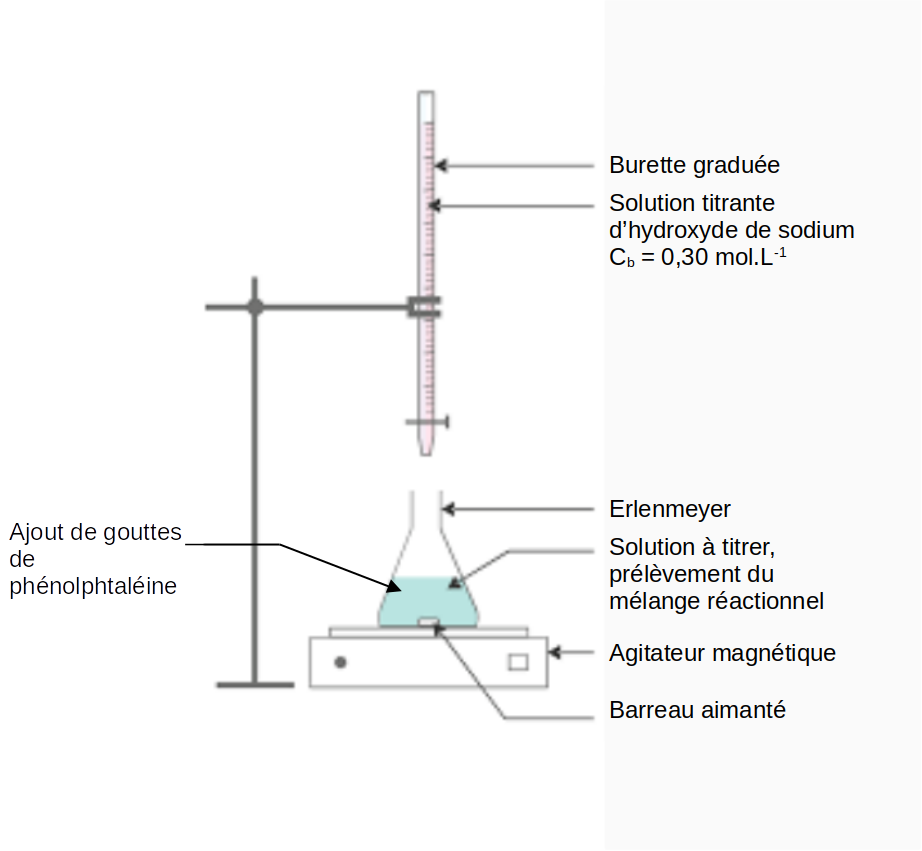
\includegraphics[scale = .3]{Ressources/TSPE_C13_AE1_Fig2.png}
	\end{minipage}
	\begin{minipage}{.3\linewidth}
		Il est nécessaire d'ajouter de l'eau distillée dans l'erlenmeyer pour avoir un volume suffisant.\\
		L'indicateur coloré de pH utilisé : \\
		Phénolphtaléine : zone de virage 8,0 - 12,0 forme acide incolore, forme basique rose
	\end{minipage}
\end{minipage}

\vspace{.5cm}
\section*{Questions préliminaires}
\begin{enumerate}
	\item Réécrire l'équation de la réaction de synthèse avec les formules demi-développées.
	\item Compléter le tableau d'avancement de la réaction de synthèse.
	\item Déterminer les quantités initiales des réactifs et les quantités maximales d'ester synthétisées et compléter les lignes correspondantes du document 2.
	\item Expliquer le rôle du titrage réalisé lorsque la synthèse est terminée.
	\item Déterminer l'équation de la réaction support de titrage et en déduire l'expression de la quantité d'acide titré.
	\item La quantité d'acide éthanoïque présente à l'état final dans le mélange 1 peut être obtenu par le calcul : $n(AH)_f = 10,8 \times n(AH)_{\text{titré}}$. Justifier ce calcul et en déduire les autres coefficients multiplicateurs.
	\item Exprimer la quantité d'ester finale en fonction des quantités $n(AH)_i$ et $n(AH)_f$.
\end{enumerate}
\section*{Exploitation des résultats}
\begin{enumerate}[resume]
	\item Compléter le tableau à l'aide de vos résultats et de ceux des autres groupes.
	\item Que peut-on conclure sur les rendements obtenus ?
\end{enumerate}
\end{document}